\section{Results and Discussion} \todo{from here forward this is incomplete}


\subsection{How can textual sentiment prediction be optimised?}

Two main methods of predicting the sentiment of input text have been analysed, using a bag-of-words method, and using machine learning approaches.

The lexicon based bag-of-words is based entirely on having an appropriate dataset to rank the words, since as Table \ref{lexicon:f1} shows, having rated VAD scores which follow a certain structure is key to obtaining good results. Dimensions like the Dominance and Arousal of a piece of text can be very subjective, and vary depending on what the data is ranging these scores from. 

The decision to use the machine learning based model for the implementation is due to having overall more stable F1 scores for each dimension, but this is only due to training and testing over the same dataset. 

To run across the whole EmoBank dataset, the bag-of-words implementation takes 182 seconds.
    
\todo{mosaic plot, adjusting the score}


\begin{figure}[ht]
\caption{Emobank data distribution with relationships. The Pearson residuals are the deviation from the expected frequency by a Pearson $X^2$ Test \cite{pearson1900x}}
\centering
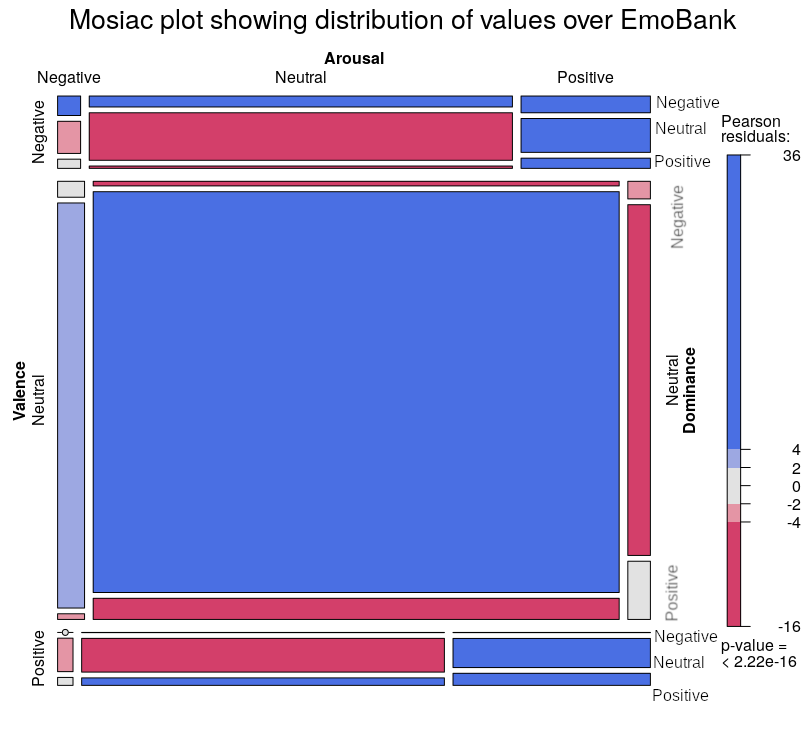
\includegraphics[scale=0.7]{graphs/mosaic_new.png}
\label{mosaic:emo}
\end{figure}

\todo{table with computation times, compare them}

\subsection{Does using more than 1 dimension to classify emotions provide more insight, and how can this be quantified?}

Getting an F1 score of \todo{this} on the model is a reasonable result, but testing whether users believe that the model is accurately predicting their moods is something that needs to be assessed. Using the built web application on conjunction we are able gain feedback from test users, asking them to input their own text and access their own Spotify data through the application to obtain a result.

Out of the 5 users that the program was tested with, 3 concluded that the song did match their emotion and 2 did not. This is a very small focus group, and for a more detailed analysis more feedback needs to be gathered, but for the purpose of gaining insight into whether the system is appropriate for answering the research question, an initial idea can be obtained.

It was decided to initially hide the calculated Ekmans emotion \todo{make sure this is mentioned earlier} from the user, so that their analysis of the result song is not influenced. 
Two users, one which agreed with the result and one that did not are studied in more detailed as follows:

\subsubsection{User A}

\begin{figure}[ht]
\caption{User A: input and output}
\centering
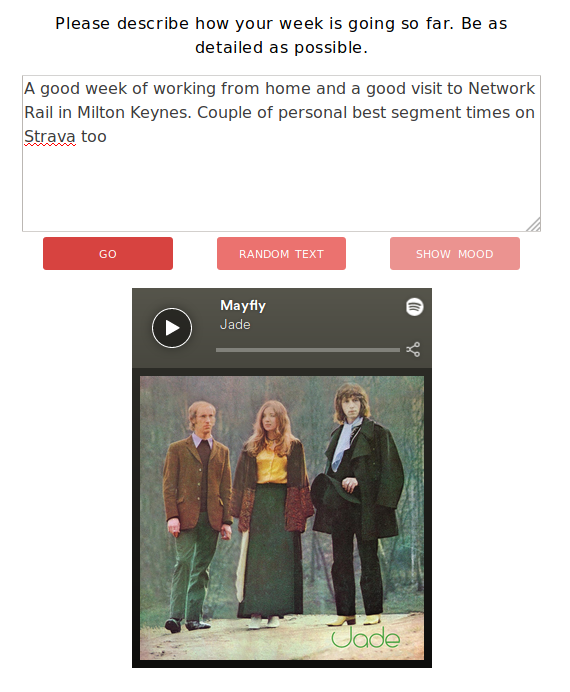
\includegraphics[scale=0.4]{implementation/malc-user.png}
\label{user:1}
\end{figure}

The first user concluded that the song matched what they had input, stating that it was upbeat and had "positive vibes". They did suggest that it would be nice to see how the song was calculated in more detail however. The calculated Ekman's emotion in this case was "Surprise", which was decided was incorrect, particularly when knowing that "Happy" was one of the options that could have been selected.

\begin{table}[h]
\centering
\begin{tabular}{|l|l|}
\hline
 Valence &  0.7\\
 Arousal &  0.6\\
 Domiance &  0.5\\
 Ekman's Emotion &  Surprise\\ \hline
\end{tabular}
\end{table}

\subsubsection{User B}

\begin{figure}[ht]
\caption{User B: input and output}
\centering
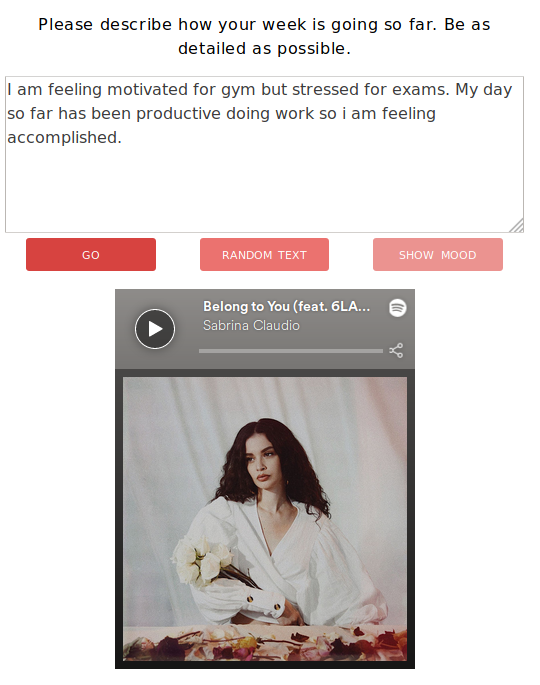
\includegraphics[scale=0.4]{implementation/jana.png}
\label{user:2}
\end{figure}

The second user concluded that the song did not match their mood, since its a very relaxed song, but they did mention that they've been listening to a lot of relaxing music recently. Other reasons why the song did not fit were also discussed, such as words such as "exams" and "work" potentially having an effect on the result.

\begin{table}[h]
\centering
\begin{tabular}{|l|l|}
\hline

 Valence &  0.6\\
 Arousal &  0.6\\
 Domiance &  0.5\\
 Ekman's Emotion &  Surprise\\ \hline
\end{tabular}
\end{table}

\subsubsection{Issues}

To be able to evoke enough emotive text from a user, the UI states "Please describe how your week is going so far. Be as detailed as possible.". This was arbitrarily chosen as just a question that does not simply have a yes or no answer, and an investigation could be made in future to find a better way of inspiring the optimal amount of input text an particularly emotive style.

All but 2 of the tests gave the result Ekman's emotion back as "Surprise", and the other two came back with "Disgust" which was incorrect every time. An explanation for this results would be because, as shown in \todo{contintue}

\begin{figure}[ht]
\caption{3d plot of the figures given in Table \ref{ekmansTable}}
\centering
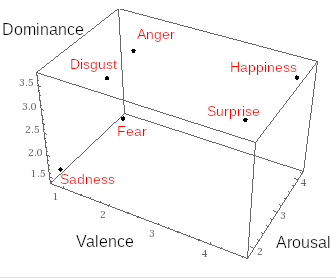
\includegraphics[scale=2]{litImgs/Ekmans3d.png}
\label{ekmans:graph}
\end{figure}

\subsection{Project Analysis}


